\section{Design}

\label{ch:met}

\subsection{Technologies used}
Firstly, the used technologies such as Spring, Mongo and Mallet will be briefly described in order
to easier follow project description later.
\subsubsection{Spring}
The Spring Framework is a comprehensive and widely used Java-based framework for building
enterprise-level applications. It provides a robust infrastructure for developing Java applications.
It simplifies the development of complex applications by promoting good design practices and
offering a suite of tools and libraries for building web applications, microservices, and
data-driven solutions. Additionally, Spring's modular architecture and extensive ecosystem
allow developers to use only the components they need, making it highly flexible and scalable.
\cite{spring}

\subsubsection{MongoDB}
MongoDB is a popular open-source, document-oriented NoSQL database designed for scalability,
flexibility, and performance. It stores data in flexible, JSON-like documents, allowing for varied
and dynamic data structures without requiring a fixed schema. MongoDB is known for its ability to handle large
volumes of data and its powerful querying and indexing capabilities. It supports a wide range of applications.
\cite{mongodb}

\subsubsection{Python}
Python is a versatile and high-level programming language known for its readability, simplicity, and extensive
standard library. It supports multiple programming paradigms, including procedural, object-oriented, and
functional programming. Python's dynamic typing and interpreted nature make it an excellent choice for rapid
application development. Python is also widely used in developing microservices due to its ease of use and
speed of development. \cite{python}

\subsubsection{Elasticsearch}
Elasticsearch is a powerful, open-source search and analytics engine designed for horizontal scalability,
reliability, and real-time search capabilities. It is built on Apache Lucene and provides a distributed, text
search engine with an HTTP web interface and schema-free JSON documents. It is commonly used for log and event
data analysis, full-text search, and real-time analytics due to its high performance, flexibility, and ability
to handle large volumes of data across distributed systems. \cite{elastic}

\subsubsection{Mallet}
MALLET (MAchine Learning for LanguagE Toolkit) is a Java-based open-source toolkit for statistical natural
language processing, particularly renowned for its implementations of topic modeling algorithms. It supports
various algorithms for discovering latent topics in large collections of text documents. MALLET provides tools
for preprocessing textual data, training topic models, and evaluating model performance. \cite{mallet}

\subsubsection{RabbitMQ}
RabbitMQ is a powerful open-source message broker that implements the Advanced Message Queuing Protocol (AMQP).
It enables seamless communication between distributed systems by acting as a mediator that facilitates the
reliable transfer of messages between applications and services. It supports various messaging patterns such
as point-to-point, publish/subscribe, and request/response. It is widely used in microservices architectures,
IoT applications, and asynchronous communication scenarios where decoupling and reliability are crucial.
\cite{rabbitmq}

\clearpage


\subsection{Design choices - overall architecture}
\begin{figure}[ht]
    \centering
    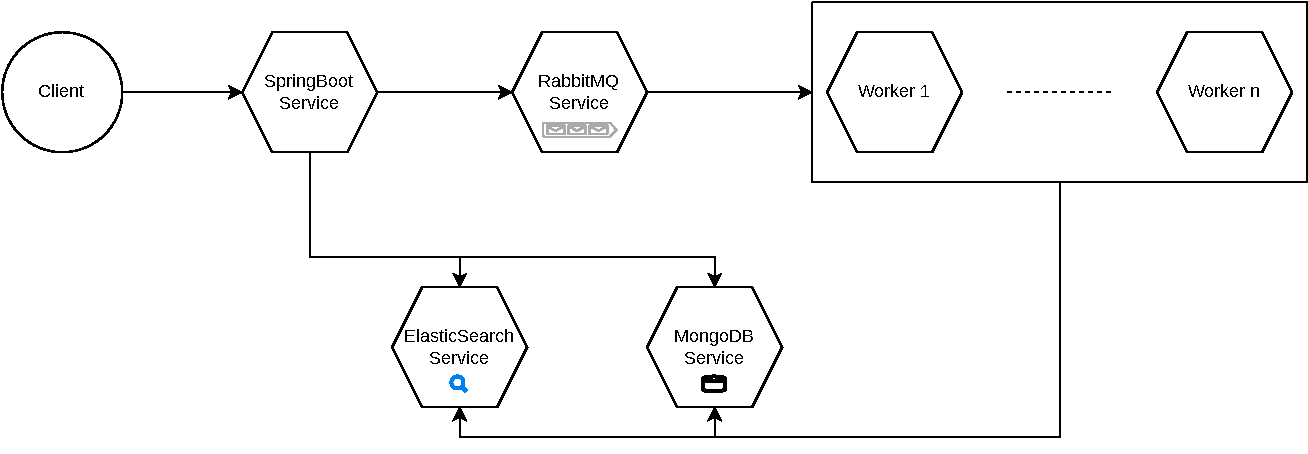
\includegraphics[width=1\linewidth] {microservices.drawio.pdf}
    \caption{Microservices}
    \label{fig:microservices}
\end{figure}

Figure~\ref{fig:microservices} shows a description of the subdivision of
the system into microservices. First of all we can see that the client can
access the application by interacting with the SpringBoot service.
This service has access to the ElasticSearch and MongoDB services and can
send messages into the queue. In the figure it is also possible to see
the workers. These microservices, that will be described in detail
later, read messages from the queue and execute the associated actions.

\clearpage

\begin{figure}[ht]
    \centering
    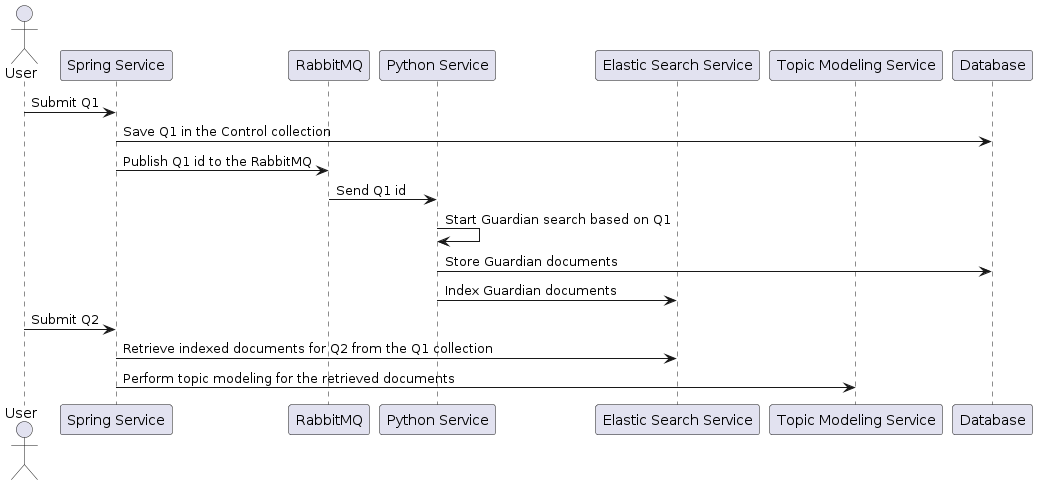
\includegraphics[width=0.7\linewidth]{figures/sequenceDiagram.png}
    \caption{Sequence diagram}
    \label{fig:seqDiagram}
\end{figure}

Figure~\ref{fig:seqDiagram} shows a sequence diagram for the whole system.
The sequence diagram starts with the user submitting Q1 to the Spring Service. The
Spring Service saves Q1 in the Control collection and publishes the Q1 id to the
RabbitMQ queue. RabbitMQ then sends the Q1 id to the Python Service, which starts a
search on Guardian based on Q1. The Python Service stores the retrieved Guardian
documents in the database and indexes them using ElasticSearchService. Later, the user
submits Q2 to the Spring Service, which retrieves the indexed documents related to Q2
from the the Q1 collection in the database and performs topic modeling on the retrieved
documents.

In the next few paragraphs, a more detailed explanation of the whole system will be provided.
Firstly, the Spring service includes a monitoring functionality, initialized by a query referred to as Q1. An
example JSON representation of Q1 is shown in Listing \ref{lst:q1}.

\begin{lstlisting}[language=json, caption={JSON representation of Q1}, label={lst:q1}]
{
  "topic": "science",
  "local_start_date": "2024-05-01",
  "local_end_date": "2024-07-01"
}
\end{lstlisting}

This query is stored in a MongoDB collection named \textit{Control}, which manages all Q1 queries.
Listing\ref{lst:q1Class} shows class structure of Q1.

\begin{lstlisting}[language=Java, caption={Class definition of QOne}, label={lst:q1Class}]
String topic;

QOneStatus status;

LocalDateTime submitted_time;
LocalDateTime finished_time;

LocalDate local_start_date;
LocalDate local_end_date;
\end{lstlisting}

The \textit{topic} field represents name of Q1, \textit{status} indicates the current processing status, which can
have the following values: SUBMITTED, PROCESSING and FINISHED. Beside that, \textit{local\_start\_date} and
\textit{local\_end\_date} are used to filter articles from the Guardian API while \textit{submitted\_date} and
\textit{finished\_date} represent the date of Q1 submission and the date when the documents fetching for Q1 is finished,
respectively. Once saved in the database, the entity's ID is published to RabbitMQ.
\newline
Concurrently, a Python service subscribes to this queue. Upon receiving the Q1 ID, it triggers fetching from
the Guardian API, setting the Q1 document status to PROCESSING. The articles retrieved from the Guardian API are saved
in MongoDB in the format shown in Listing \ref{lst:article}.

\begin{lstlisting}[language=json, caption={JSON representation of a Guardian Article}, label={lst:article}]
{
    "title": title,
    "content" : content,
    "guardian_id" : guardian_id,
    "web_date": web_date
}
\end{lstlisting}

The \textit{title} and \textit{content} fields represent title and contect of an article respectively whereas
\textit{guardian\_id} and \textit{web\_date} represent guardian id and date of publishing an article. Each article
is subsequently indexed and stored as a JSON object in the Elasticsearch server.

For the second query, Q2, a user requests \textit{k} topics. This requires the Q1 ID as a parameter. For instance,
if Q1 was about \textit{Science}, and related articles are stored in the database, a subsequent Q2 query like
\textit{Nuclear war} expects to retrieve \textit{k} topics based on that subset of documents.

\section{Design choices - per service}
This section presents the design choices for each service. 
\subsection{Design for Spring service}

One of the services in our application is a Spring service, which is responsible for receiving all user requests,
saving Q1 in the database, pushing Q1's ID to RabbitMQ, retrieving documents from the ElasticSearch server, and
performing the topic modeling part. Figure \ref{fig:spring-structure} shows the structure of the Spring service. In the chapter 
\ref {ch:motivation} we will discuss design principles we followed and a reason behind that.

\begin{figure}[ht]
  \centering
  \begin{forest}
    for tree={
      font=\ttfamily,
      grow=east,
      parent anchor=east,
      child anchor=west,
      edge path={
        \noexpand\path [draw, \forestoption{edge}] (!u.parent anchor) -- ++(5pt,0) |- (.child anchor)\forestoption{edge label};
      },
      l sep=15pt,
      s sep=15pt,
    }
    [awesomemodeling
      [controllers]
      [services]
      [repositories]
      [enums]
      [entities]
      [dtos]
      [AwesomemodelingApplication.java]
    ]
  \end{forest}
  \caption{Folder structure of the Spring service}
  \label{fig:spring-structure}
\end{figure}

\subsection{APIs}
Our application exposes different endopoints to perform all the functionalities described
in Figure \ref{fig:flow}. In the following subsections, the request and response bodies indicate
the type related to each field.

\subsubsection{GET /q1}
Retrieve a list of all the QOne objects saved in the database \\\\
\textbf{Request}
\begin{itemize}
  \item \textbf{URL:}
  \begin{quote}
    \url{/q1}
  \end{quote}
  \item \textbf{Method:} GET
\end{itemize}\leavevmode\newline
\textbf{Response}
\begin{itemize}
  \item \textbf{Status Code:} 200 OK
  \item \textbf{Body:}
    \begin{lstlisting}
      [
        {
          "id": "string",
          "topic": "string",
          "status": "string",
          "submitted_time": "datetime",
          "finished_time": "datetime",
          "local_start_date": "date",
          "local_end_date": "date"
        },
        ...
      ]
    \end{lstlisting}
\end{itemize}

\subsubsection{POST /q1}
Create a new QOne object \\\\
\textbf{Request}
\begin{itemize}
  \item \textbf{URL:}
  \begin{quote}
    \url{/q1}
  \end{quote}
  \item \textbf{Method:} POST
  \item \textbf{Headers:}
  \begin{itemize}
    \item \textbf{Content-Type:} application/json
  \end{itemize}
  \item \textbf{Body:}
    \begin{lstlisting}
      {
        "topic": "string",
        "local_start_date": "date",
        "local_end_date": "date"
      }
    \end{lstlisting}
\end{itemize}\leavevmode\newline
\textbf{Response}
\begin{itemize}
  \item \textbf{Status Code:} 201 CREATED
  \item \textbf{Body:}
    \begin{lstlisting}
      [
        {
          "id": "string",
          "topic": "string",
          "status": "string",
          "submitted_time": "datetime",
          "finished_time": "datetime",
          "local_start_date": "date",
          "local_end_date": "date"
        }
      ]
    \end{lstlisting}
\end{itemize}\leavevmode\newline
\textbf{Errors}
\begin{itemize}
  \item \textbf{500 Internal Server Error}: An error occurred while connecting to RabbitMQ
\end{itemize}

\subsubsection{GET /q1/[QOneID]}
Retrieve the QOne object specified by \verb|QOneID| \\\\
\textbf{Request}
\begin{itemize}
  \item \textbf{URL:}
  \begin{quote}
    \url{/q1/[QOneID]}
  \end{quote}
  \item \textbf{Method:} GET
\end{itemize}\leavevmode\newline
\textbf{Response}
\begin{itemize}
  \item \textbf{Status Code:} 200 OK
  \item \textbf{Body:}
    \begin{lstlisting}
      [
        {
          "id": "[QOneID]",
          "topic": "string",
          "status": "string",
          "submitted_time": "datetime",
          "finished_time": "datetime",
          "local_start_date": "date",
          "local_end_date": "date"
        }
      ]
    \end{lstlisting}
\end{itemize}\leavevmode\newline
\textbf{Errors}
\begin{itemize}
  \item \textbf{404 Not Found}: the specified QOne does not exist
\end{itemize}

\subsubsection{GET /q1/[QOneID]/q2}
Retrieve the themes related to \verb|QOneID| \\\\
\textbf{Request}
\begin{itemize}
  \item \textbf{URL:}
  \begin{quote}
    \url{/q1/[QOneID]}
  \end{quote}
  \item \textbf{Parameters:}
    \begin{itemize}
      \item \textbf{query} (mandatory): a query (Q2) related to Q1 on which performing topic modeling
      \item \textbf{k} (mandatory): the desired number of topics
    \end{itemize}
  \item \textbf{Method:} GET
\end{itemize}\leavevmode\newline
\textbf{Response}
\begin{itemize}
  \item \textbf{Status Code:} 200 OK
  \item \textbf{Body:}
    \begin{lstlisting}
      {
        "topics": [
          {
            "topic": [
              "string",
              "string",
              "string",
              "string",
              "string",
              "string",
              "string",
              "string",
              "string",
              "string"
            ]
          },
          ...
        ]
      }
    \end{lstlisting}
\end{itemize}\leavevmode\newline
\textbf{Errors}
\begin{itemize}
  \item \textbf{404 Not Found}: the specified QOne does not exist
  \item \textbf{500 Internal Server Error}: topic retrieval failed
\end{itemize}

\subsection{Design for Python service}
Another service that is part of our application is the Python service called \textit{downindex}, which is responsible for listening to incoming messages in \textit{RabbitMQ}, fetching articles from the \textit{Guardian API}, and indexing them using \textit{ElasticSearch}. The structure of this service is very simple and is shown in Figure \ref{fig:python-structure}. \textit{main.py} holds all the business logic of the service, while \textit{requirements.txt} lists all the required dependencies.

\begin{figure}[ht]
  \centering
  \begin{forest}
    for tree={
      font=\ttfamily,
      grow=east,
      parent anchor=east,
      child anchor=west,
      edge path={
        \noexpand\path [draw, \forestoption{edge}] (!u.parent anchor) -- ++(5pt,0) |- (.child anchor)\forestoption{edge label};
      },
      l sep=15pt,
      s sep=15pt,
    }
    [downindex
      [main.py]
      [requirements.txt]
    ]
  \end{forest}
  \caption{Folder structure of the Python service}
  \label{fig:python-structure}
\end{figure}

\clearpage

\subsection{Message Queue}

\begin{figure}[ht]
    \centering
    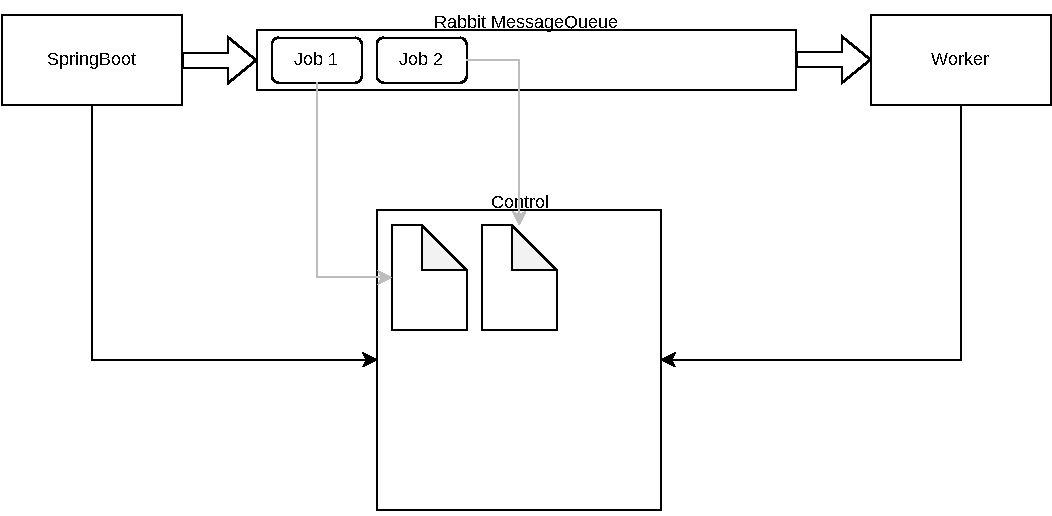
\includegraphics[width=1\linewidth] {queue.drawio}
    \caption{Queue}
    \label{fig:queue}
\end{figure}

Figure~\ref{fig:queue} shows the architecture of the communication between
the SpringBoot service (which is the service the user can interact with)
and the worker nodes.

In this example only one worker it is present but
the same would apply if more than one worker was active. In that case the only
difference would be that the messages in the queue could be received by different
workers.

The process goes as follows: the SpringBoot application creates a document
in the \textit{control} collection containing all the information that the
worker needs to know to perform the action. In our system the only action
that is submitted in the queue is the download and index of a topic.
The Spring microservice then posts a message in the queue containing the
id of the document.

This message will be then received by one of the workers. The first action
that the worker does is retrieving the associated control document from the
collection. Then it writes on the document that the action is being processed
(so that an user can see that the system is working on its request) and starts
performing it.

When the job is completed, the worker writes on the document that it is done.

